% ==============================================================================
% Resumo Conciso das Alterações Metodológicas e Interpretação das Novas Figuras
% ==============================================================================
\documentclass[12pt,a4paper]{article}
\usepackage[utf8]{inputenc}
\usepackage[T1]{fontenc}
\usepackage[brazilian]{babel}
\usepackage{graphicx}
\usepackage{amsmath,amssymb}
\usepackage{booktabs}
\usepackage{geometry}
\geometry{a4paper, margin=2.5cm}
\usepackage{lmodern}
\usepackage{microtype}
\usepackage{xcolor}
\usepackage[colorlinks=true,allcolors=blue!80!black]{hyperref}

% Caminho para encontrar os PDFs das figuras na pasta Tese
\graphicspath{{../Tese/}{./}}

\title{\textbf{Refinamento Metodológico e Análise Alométrica por Bacia}\\[0.5ex]
\large Resumo Conciso das Alterações e Interpretação das Novas Figuras}
\author{Thiago de Oliveira Sampaio}
\date{\today}

\begin{document}
\maketitle

\section{Refinamento Metodológico e Análise Alométrica por Bacia}

Com base nas diretrizes metodológicas estabelecidas para o domínio continental da América do Norte até o Canal do Panamá ($[-125^\circ\text{O}, 7^\circ\text{N}, -65^\circ\text{O}, 50^\circ\text{N}]$), o pipeline de cruzamento entre bacias hidrográficas (GEBCO/IPBA), aglomerados urbanos (GPW v4/CCA) e microplásticos costeiros (NOAA/\textit{Nurdle Patrol}) recebeu quatro aprimoramentos analíticos e visuais:

\begin{enumerate}
    \item \textbf{Integração entre a calibração de Zipf (CCA) e a alometria por bacia (\texttt{pop\_urbana} vs.\ \texttt{pop\_total}):}
    Os parâmetros críticos do \textit{City Clustering Algorithm} ($D^* = 1010\text{ hab/km}^2$ e $\ell = 1700\text{ m}$), calibrados pela invariância de escala da Lei de Zipf ($\alpha \approx 1$), definem as manchas urbanas que são seccionadas pelas linhas de cumeada de cada bacia. Além da população total residente na bacia (\texttt{pop\_total}), passou-se a avaliar explicitamente a população urbana fatiada por bacia (\texttt{pop\_urbana}), elevando a correlação de postos de Spearman com a concentração de microplásticos de $\rho_s = 0{,}48$ para $\rho_s = 0{,}52$ ($R \le 38\text{ km}$) e de $\rho_s = 0{,}61$ para $\rho_s = 0{,}63$ ($R \le 5\text{ km}$).

    \item \textbf{Resolução física do pixel da foz ($R = 5\text{ km}$) vs.\ escala sub-pixel ($R = 1\text{ km}$):}
    Como o relevo GEBCO é reamostrado em células de $2' \times 2'$ ($\sim 3{,}7\text{ km}$ de lado, diagonal de $\sim 5{,}2\text{ km}$), impor um raio estrito de $R = 1\text{ km}$ exige precisão sub-pixel inferior à resolução da grade hidrográfica, retendo apenas $n = 3$ bacias com contagem positiva (\textit{San Jacinto}, \textit{San Gabriel} e \textit{Baffin Bay}). Ao adotar a escala física de $\sim 1$ pixel da foz ($R \le 5\text{ km}$), o conjunto amostral salta para $n = 17$ bacias independentes (17 estações distintas, sem sobreposição), viabilizando o ajuste alométrico na zona estuarina imediata.

    \item \textbf{Decomposição aditiva do acoplamento com a área da bacia:}
    Para a carga estimada na foz ($Y_{\text{carga}} = \text{Concentração} \times \text{Área}$), a transformação logarítmica implica $\log_{10}(\text{Conc} \times \text{Área}) = \log_{10}(\text{Conc}) + \log_{10}(\text{Área})$. Pela linearidade do estimador de mínimos quadrados ordinários (MQO), o expoente alométrico total decompõe-se exatamente em:
    \begin{equation}
        \beta_{\text{carga}} = \beta_{\text{conc}} + \beta_{\text{área}}
    \end{equation}
    Separou-se, assim, o efeito intrínseco da concentração ($\beta_{\text{conc}} = 0{,}28$) do efeito geométrico de escala da área de drenagem ($\beta_{\text{área}} = 0{,}57$), resultando em $\beta_{\text{carga}} = 0{,}85$ (regime sublinear frente à referência isométrica $\beta = 1{,}00$).

    \item \textbf{Validação hidrológica continental:}
    As grandes bacias delineadas de forma não supervisionada pelo IPBA reproduzem com erro inferior a $2{,}5\%$ as áreas oficiais do USGS e da CONAGUA, incluindo os sistemas do Mississippi ($3{,}15 \times 10^6\text{ km}^2$ vs.\ $3{,}22 \times 10^6\text{ km}^2$ oficial; $-2{,}1\%$), São Lourenço ($1{,}37 \times 10^6\text{ km}^2$; $+2{,}3\%$), Rio Grande ($8{,}50 \times 10^5\text{ km}^2$; $-2{,}3\%$), Lerma--Santiago ($-1{,}9\%$) e Balsas ($-0{,}3\%$).
\end{enumerate}

% ------------------------------------------------------------------------------
\subsection{Interpretação das Figuras Atualizadas}

\begin{figure}[htbp]
    \centering
    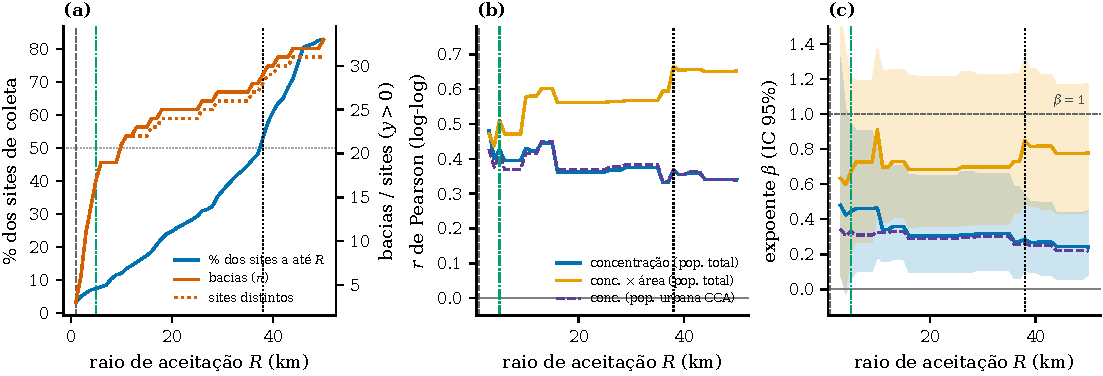
\includegraphics[width=\textwidth]{figuras/varredura_raio.pdf}
    \caption{Varredura do raio de aceitação $R$ entre $1\text{ km}$ e $50\text{ km}$ a partir do pixel de foz (\textit{sink}) de cada bacia principal. \textbf{(a)} Percentual acumulado de estações do \textit{Nurdle Patrol} capturadas (eixo esquerdo) e número de bacias e estações distintas com medição positiva (eixo direito). As linhas verticais destacam $R = 1\text{ km}$ (sub-pixel, $n=3$), $R = 5\text{ km}$ ($\sim 1$ pixel do DEM, $n=17$) e $R_{\text{maioria}} = 38\text{ km}$ ($\ge 50\%$ dos sites, $n=29$). \textbf{(b)} Coeficiente de correlação de Pearson ($r$ em escala log-log) para concentração pura (azul), concentração por população urbana do CCA (roxo tracejado) e carga total $\text{Conc} \times \text{Área}$ (laranja). \textbf{(c)} Evolução do expoente alométrico $\beta$ e respectivo intervalo de confiança de $95\%$ via \textit{bootstrap}, comparado ao limiar de isometria ($\beta = 1$).}
    \label{fig:varredura_raio}
\end{figure}

A \textbf{Figura~\ref{fig:varredura_raio}} demonstra a estabilidade dos parâmetros de escala ao longo da varredura espacial de $1\text{ a }50\text{ km}$. A partir da escala de resolução do pixel ($R \ge 5\text{ km}$), tanto a correlação quanto o expoente $\beta$ estabilizam-se em patamares estatisticamente significativos, demonstrando que a lei de escala não é um artefato da escolha arbitrária de um raio fixo.

\begin{figure}[htbp]
    \centering
    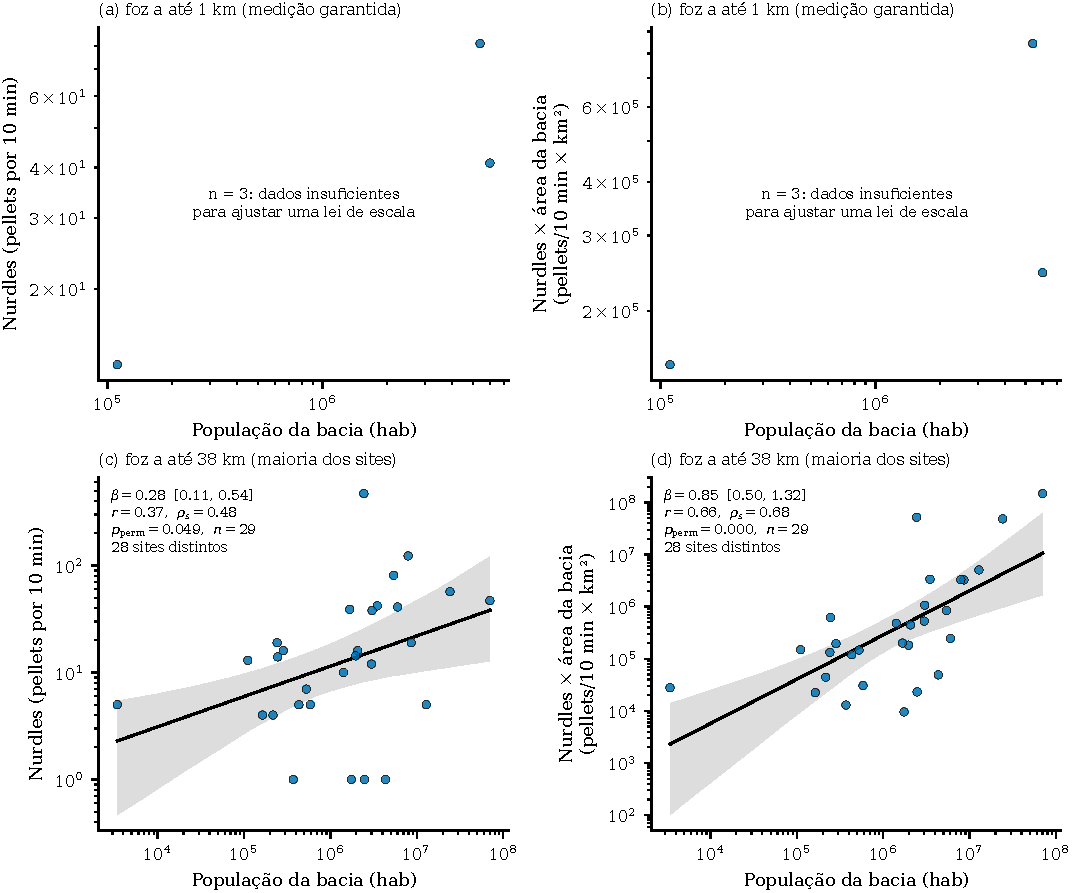
\includegraphics[width=\textwidth]{figuras/dispersao_pop_lixo.pdf}
    \caption{Relações de escala alométrica ($y = c\,x^\beta$) entre população da bacia hidrográfica e microplásticos na foz. \textbf{(a, b)} Zona imediata da foz ($R \le 5\text{ km}$, equivalente a $\sim 1$ pixel da grade do GEBCO; $n = 17$ bacias e $17$ sites distintos), destacando com estrelas douradas as $n = 3$ bacias com coleta a $d \le 1\text{ km}$ (\textit{San Jacinto}, \textit{San Gabriel} e \textit{Baffin Bay}). \textbf{(c, d)} Raio de maioria amostral ($R \le 38\text{ km}$; $n = 29$ bacias e $28$ sites distintos). Os painéis à esquerda \textbf{(a, c)} avaliam a concentração bruta ($\text{pellets/10 min}$) e os painéis à direita \textbf{(b, d)} avaliam o indicador de carga ($\text{Concentração} \times \text{Área}$), incluindo a linha pontilhada de referência isométrica ($\beta = 1$) e a decomposição aditiva $\beta_{\text{conc}} + \beta_{\text{área}}$.}
    \label{fig:dispersao_pop_lixo}
\end{figure}

Na \textbf{Figura~\ref{fig:dispersao_pop_lixo}}, observa-se que na zona imediata da foz ($R \le 5\text{ km}$, painéis \textbf{a} e \textbf{b}), a concentração apresenta forte correlação monotônica com a população ($\rho_s = 0{,}61$ para população total e $\rho_s = 0{,}63$ para população urbana do CCA), enquanto a carga total escala com $\beta = 0{,}67$ ($r = 0{,}51$, $\rho_s = 0{,}65$, $p_{\text{perm}} = 0{,}039$). No raio da maioria dos pontos ($R \le 38\text{ km}$, painéis \textbf{c} e \textbf{d}), a concentração mantém regime sublinear ($\beta = 0{,}28$, $p_{\text{perm}} = 0{,}049$) e a carga total atinge $\beta = 0{,}85$ ($\text{IC}_{95\%} = [0{,}50;\ 1{,}32]$, $r = 0{,}66$, $\rho_s = 0{,}68$, $p_{\text{perm}} < 0{,}001$), decompondo-se em $\beta_{\text{conc}} = 0{,}28$ e $\beta_{\text{área}} = 0{,}57$.

\begin{figure}[htbp]
    \centering
    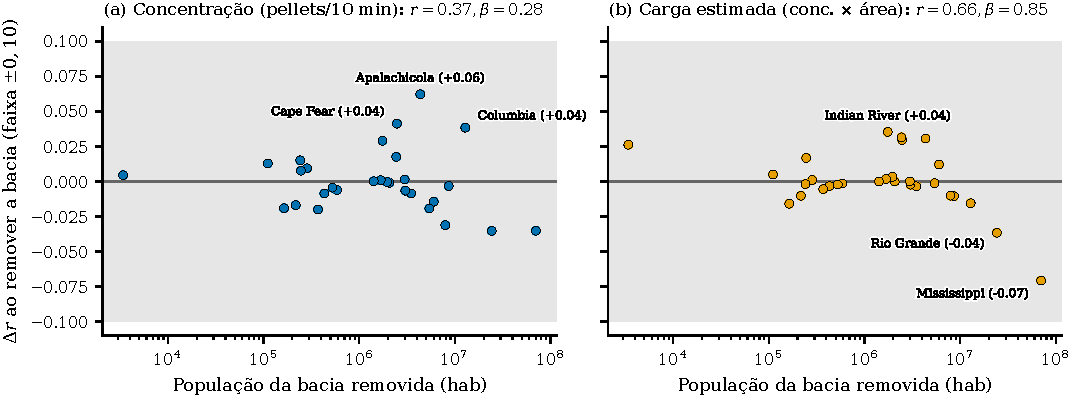
\includegraphics[width=\textwidth]{figuras/leave_one_out.pdf}
    \caption{Análise de sensibilidade \textit{leave-one-out} (jackknife) para $R_{\text{maioria}} = 38\text{ km}$ ($n = 29$), exibindo o deslocamento $\Delta r = r_{\text{sem } i} - r_{\text{todas}}$ na correlação de Pearson após a remoção individual de cada bacia hidrográfica: \textbf{(a)} concentração ($\text{pellets/10 min}$) e \textbf{(b)} carga estimada ($\text{Concentração} \times \text{Área}$). A faixa cinza delimita a zona de estabilidade $|\Delta r| \le 0{,}10$.}
    \label{fig:leave_one_out}
\end{figure}

Por fim, a \textbf{Figura~\ref{fig:leave_one_out}} comprova a robustez da regressão frente a valores extremos (\textit{outliers}): mesmo a remoção individual de bacias continentais como as dos rios \textit{Mississippi} ($70{,}2\text{ milhões}$ de habitantes, $\Delta r = -0{,}07$), \textit{Rio Grande} ($24{,}2\text{ milhões}$, $\Delta r = -0{,}04$) ou \textit{Colorado-TX} (maior concentração registrada, $471\text{ pellets/10 min}$) mantém a variação de $r$ estritamente contida no intervalo $[-0{,}07, +0{,}06]$, dentro da banda de estabilidade de $\pm 0{,}10$.

\end{document}
